%!TEX root = ../../root.tex

Every task we have seen so far relied on the Euclidean domain. However, many scientific fields study data with an underlying structure that is a non-Euclidean space: think of social networks represented as graphs, or meshed surfaces in computer graphics.

\paragraph{Geometric deep learning vs manifold learning}

Notice that this setting is different from \emph{manifold learning}, in which we seek for a manifold that justifies a given set of data. In fact, this data can still be represented as vectors in a (possibly high-dimensional) embedding space, and seeking a manifold is just a way for us to learn more accurate mappings (charts) from the latent space to the data space, subset of the embedding space. 

On the other hand, this is not possible for data that \emph{intrinsically} lives in a non-Euclidean domain such as a graph, because the information is encoded both as data on the domain (features of a certain user in a social network), but also in the \emph{domain structure} (connections between users) itself, while in a Euclidean domain we care only about the information encoded by the data, since the domain has a shared, grid-like, flat structure for every possible type of data (\textit{e.g.} images or audio signals).

\begin{figure}[H]
    \centering
    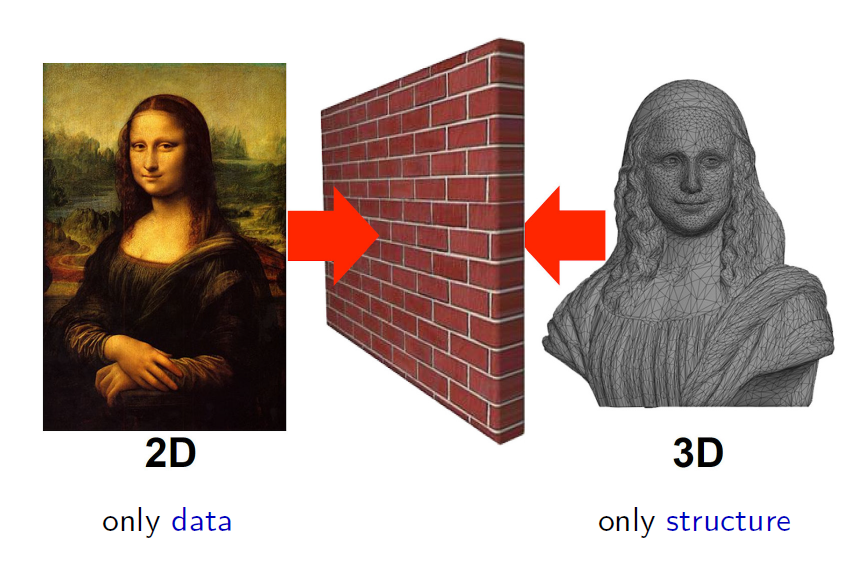
\includegraphics[width=.7\textwidth]{figures/12/monalisa-domain.png}
    \caption{On the left, we have only data, i.e. the intensity values for the three channels for every pixel, that can be expressed as a vector-to-vector function. On the right, we have only the structure, but that still encodes relevant information, even without the data. We want to capture both.}
\end{figure}

So in this new settings we are not trying to \emph{learn} a manifold, we already know the geometry of the manifold, or of the graph, the problem is that a great deal of the information of the data comes from this known, but hard to represent, geometric structure.

Another critical aspect to consider in geometric deep learning is the dynamic nature of the domains, so for example to make prediction on a social network we don't need to have all the information of how the graph changes over time (new social connections), instead for surfaces probably the information that we care about is encoded in how the object transforms.
\begin{figure}[H]
	\centering
	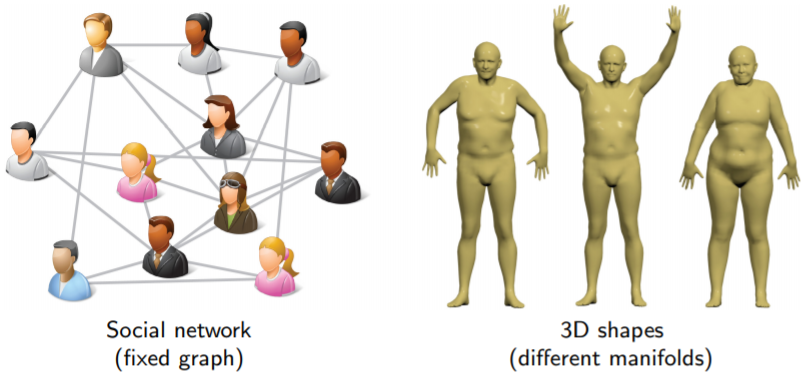
\includegraphics[width=.8\textwidth]{12/6_46}
	\caption{Static vs dynamic domain.}\label{fig:domain}	
\end{figure}
